\documentclass{beamer}
\usepackage{caption}
\usepackage{listings}
\usepackage[official]{eurosym}
% Remove the navigation buttons at the bottom right of each slide.
\setbeamertemplate{navigation symbols}{}
% Set bulletpoints to circles.
\setbeamertemplate{itemize items}[circle]

\title{Intro to Git}
\author{Netsoc}
% Remove the date.
\date{}
\begin{document}
\frame{\titlepage}

\section{Goals}
\begin{frame}
\frametitle{Goals}
\begin{itemize}
\item Show you the 10\% of Git that can do 90\% of the work
\item Slides \& practical demonstration
\item Questions \& Answers
\end{itemize}
\end{frame}

\section{Git}
\begin{frame}
\frametitle{Git}
\begin{itemize}
\item Version Control System (VCS)
\begin{itemize}
\item Keep track of changes in files over time
\item Track who changed what, when
\item Help multiple people work on the same files at the same time
\item Detect and sometimes resolve conflicts automatically
\end{itemize}
\item Created by Linus Torvalds in 2005 for Linux Kernel development
\item Command-line program, available on Linux, Mac and Windows
\item Free and Open-Source
\item https://git-scm.com/
\end{itemize}
\end{frame}

\begin{frame}
\begin{figure}
\begin{center}
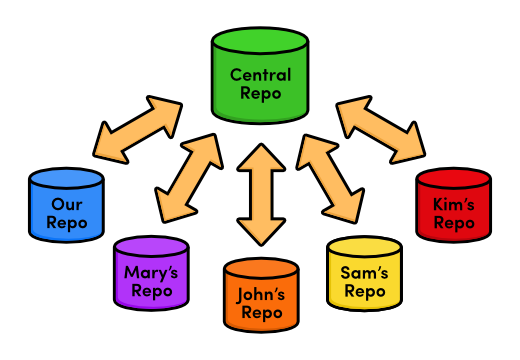
\includegraphics[scale=0.7]{centralised}
\caption{http://rypress.com/tutorials/git/media/8-7.png}
\end{center}
\end{figure}
\end{frame}

\begin{frame}
\frametitle{Github}
\begin{itemize}
\item A website for hosting git repositories
\item It's free
\item The user interface is great
\item Issue tracker, search function, can "star" and follow repositories
\end{itemize}
\end{frame}

\begin{frame}
\begin{figure}
\begin{center}
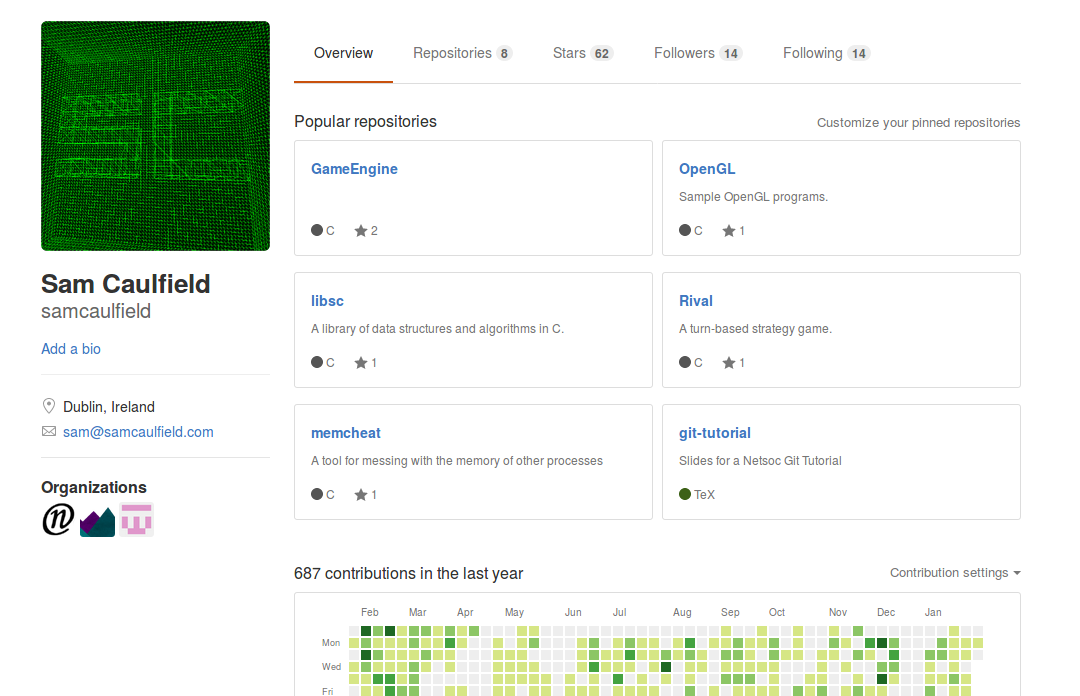
\includegraphics[scale=0.3]{githubmain}
\end{center}
\end{figure}
\end{frame}

\section{Getting a repository}
\begin{frame}
\frametitle{Getting a repository}
\begin{itemize}
\item Need to create or get a copy of the repository to begin working
\item to create: git init
\end{itemize}
\begin{figure}
\begin{center}
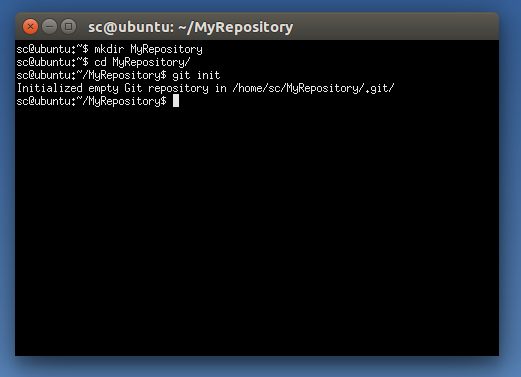
\includegraphics[scale=0.5]{gitinit}
\end{center}
\end{figure}
\end{frame}

\section{Getting a repository}
\begin{frame}
\frametitle{Getting a repository}
\begin{itemize}
\item If you're not starting from scratch, need to get it from somewhere
\item to copy from somewhere else: git clone
\end{itemize}
\begin{figure}
\begin{center}
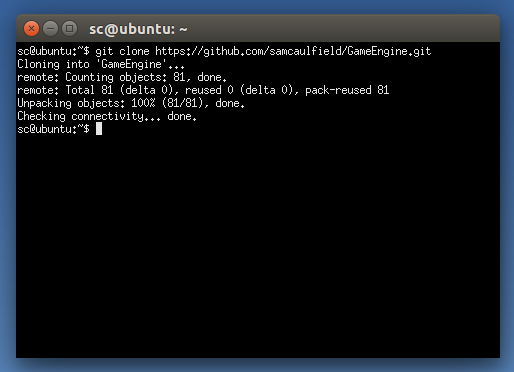
\includegraphics[scale=0.5]{gitclone}
\end{center}
\end{figure}
\end{frame}

\section{Modifying your own repository}
\begin{frame}
\frametitle{Adding things to your repository}
\begin{itemize}
\item Git has the concept of a "staging area"
\item By default changes to files are unstaged
\item You manually add files to the staging area
\item Then you can confirm a subset of the changes (commit)
\end{itemize}
\end{frame}

\begin{frame}
\begin{figure}
\begin{center}
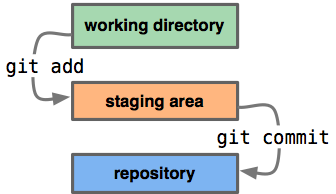
\includegraphics[scale=1.4]{stagingareadiagram}
\caption{http://codingdomain.com/git/partial-commits/git-staging-area.png}
\end{center}
\end{figure}
\end{frame}

\begin{frame}
\begin{figure}
\begin{center}
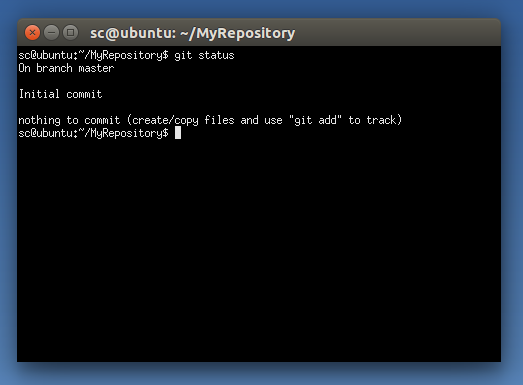
\includegraphics[scale=0.5]{gitstatus0}
\end{center}
\end{figure}
\end{frame}

\begin{frame}
\begin{figure}
\begin{center}
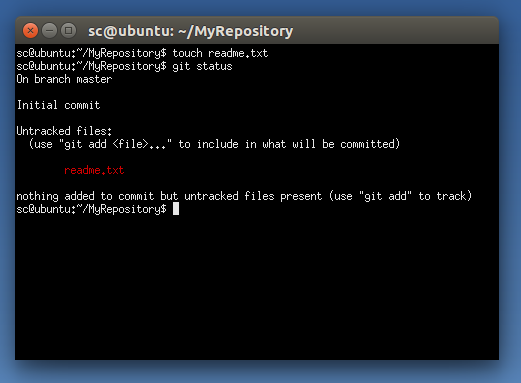
\includegraphics[scale=0.5]{gitstatus1}
\end{center}
\end{figure}
\end{frame}

\begin{frame}
\frametitle{Staging files}
\begin{itemize}
\item Use the "git add" command (same as "git stage")
\end{itemize}
\begin{figure}
\begin{center}
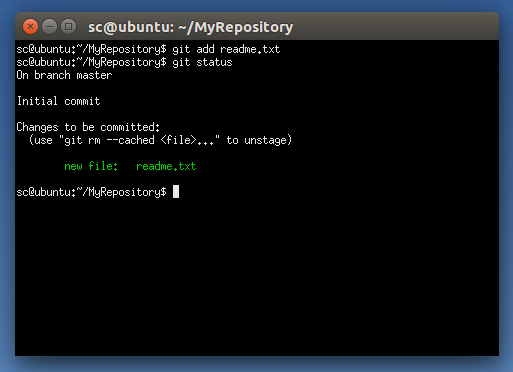
\includegraphics[scale=0.5]{gitadd0}
\end{center}
\end{figure}
\end{frame}

\section{Staging files}
\begin{frame}
\begin{itemize}
\item You can add multiple files with wildcard (git add *)
\item This often goes wrong
\item .exe .bin .o .class .so etc.
\item .gitignore file can mitigate this
\end{itemize}
\end{frame}

\section{Syncing your changes with other people}
\begin{frame}
\end{frame}

\section{Workflow}
\begin{frame}
\end{frame}

\end{document}

